% crea il CAPITOLO
\chapter{Alchemist}
% imposta l'intestazione di pagina
\lhead[\fancyplain{}{\bfseries\thepage}]{\fancyplain{}{\bfseries\rightmark}}
% mette i numeri arabi
%\pagenumbering{arabic}

Per la realizzazione dell'ambiente per il progetto di tesi è stato scelto il simulatore Alchemist, poichè fornisce già una struttura ed un meta-modello solido e utilizzabile. Nel capitolo viene mostrato Alchemist attraverso le funzionalità e ciò che lo compone. Successivamente è presentata una serie di peculiarità di questo strumento che saranno approfondite più avanti nel documento.

%----------------------------
\section{Descrizione Alchemist}
Alchemist è un simulatore per il calcolo pervasivo, aggregato e ispirato alla natura. Esso fornisce un ambiente di simulazione sul quale è possibile sviluppare nuove incarnazioni, cioè nuove definizioni di modelli implementati su di esso. Ad oggi sono disponibili le funzionalità per:
\begin{itemize}
\item simulare un ambiente bidimensionale;
\item simulare mappe del mondo reale, con supporto alla navigazione e importazione di tracciati in formato gpx;
\item simulare ambienti indoor importando immagini in bianco e nero;
\item eseguire simulazioni biologiche utilizzando reazioni in stile chimico;
\item eseguire programmi Protelis, Scafi, SAPERE (scritti in un linguaggio basato su tuple come LINDA).
\end{itemize}

\subsection{Meta-modello}
Il meta-modello di Alchemist può essere compreso osservando la figura \ref{fig:alchemistModel}.
%crea l'ambiente figura;
\begin{figure}[h] % [h] sta per here, cioè la figura va qui
\begin{center} % centra nel mezzo della pagina la figura
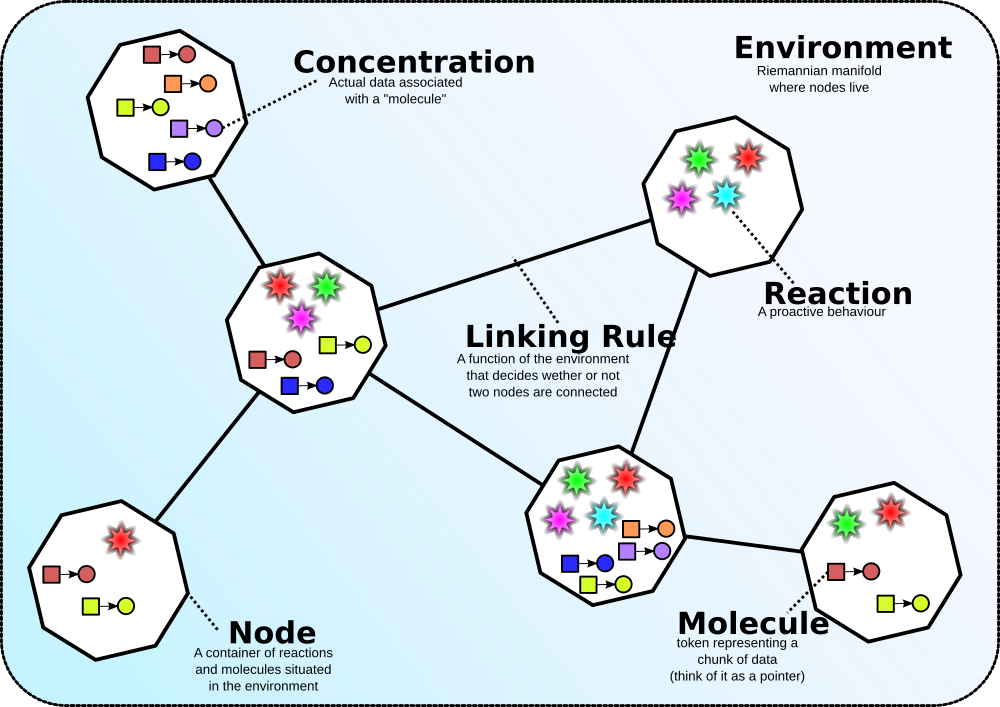
\includegraphics[width=12.5cm]{images/AlchemistModel.png} % inserisce una figura larga 12.5cm
% inserisce la legenda ed etichetta la figura con \label{fig:prima}
\caption[Illustrazione meta-modello di Alchemist]{Illustrazione meta-modello di Alchemist} \label{fig:alchemistModel}
\end{center}
\end{figure}

L'\textbf{\textit{Environment}} è l'astrazione dello spazio ed è anche l'entità più esterna che funge da contenitore per i nodi. Conosce la posizione di ogni nodo nello spazio ed è quindi in grado di fornire la distanza tra due di essi e ne permette inoltre lo spostamento.

\`E detta \textbf{\textit{Linking rule}} una funzione dello stato corrente dell'environemnt che associa ad ogni nodo un \textbf{\textit{Vicinato}}, il quale è un entità composta da un nodo centrale e da un set di nodi vicini.

Un \textbf{\textit{Nodo}} è un contenitore di molecole e reazioni che è posizionato all'interno di un environment.

La \textbf{\textit{Molecola}} è il nome di un dato, paragonabile a quello che rappresenta il nome di una variabile per i linguaggi imperativi.
Il valore da associare ad una molecola è detto \textbf{\textit{Concentrazione}}.

%crea l'ambiente figura;
\begin{figure}[h] % [h] sta per here, cioè la figura va qui
\begin{center} % centra nel mezzo della pagina la figura
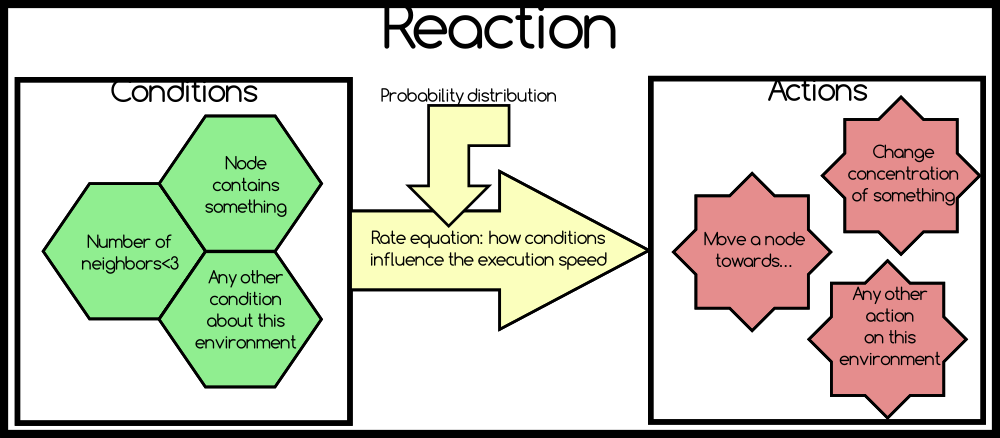
\includegraphics[width=14cm]{images/AlchemistReaction.png} % inserisce una figura larga 12.5cm
% inserisce la legenda ed etichetta la figura con \label{fig:prima}
\caption[Illustrazione modello reazione di Alchemist]{Illustrazione modello reazione di Alchemist} \label{fig:alchemistReaction}
\end{center}
\end{figure}

Una \textbf{\textit{Reazione}} è un qualsiasi evento che può cambiare lo stato dell'environment ed è definita tramite una distribuzione temporale, una lista di condizioni e una o più azioni.
\\La frequenza con cui avvengono dipende da:
\begin{itemize}
\item un parametro statico di frequenza;
\item il valore di ogni condizione;
\item un'equazione di frequenza che combina il parametro statico e il valore delle condizioni restituendo la frequenza istantanea;
\item una distribuzione temporale.
\end{itemize}
Ogni nodo contiene un set di reazioni che può essere anche vuoto.

Per comprendere meglio il meccanismo di una reazione si può osservare la figura \ref{fig:alchemistReaction}.

Una \textbf{\textit{Condizione}} è una funzione che prende come input l'environment corrente e restituisce come output un booleano e un numero. Se la condizione non si verifica, le azioni associate a quella reazione non saranno eseguite. In relazione a parametri di configurazione e alla distribuzione temporale, una condizione potrebbe influire sulla velocità della reazione.

La \textbf{\textit{Distribuzione temporale}} indica il numero di eventi, in un dato intervallo di tempo, generati da Alchemist e che innescano la verifica delle condizioni che possono portare alla potenziale esecuzione delle azioni.

Un'\textbf{\textit{Azione}} è la definizione di una serie di operazioni che modellano un cambiamento nel nodo o nell'environment.

In Alchemist un'incarnazione è un'istanza concreta del meta-modello appena descritta e che implementa una serie di componenti base come: la definizione di una molecola e del tipo di dati della concentrazione, un set di condizioni, le azioni e le reazioni. Incarnazioni diverse possono modellare universi completamente differenti.


\section{Aspetti principali in Alchemist}
Alchemist è uno strumento molto esteso e che può offrire tantissime possibilità se lo si conosce e si è in grado di padroneggiarlo.
La conoscenza iniziale di questo ambiente era però praticamente nulla e, quindi è stato necessario impiegare del tempo per riuscire a padroneggiare i meccanismi di base, tra cui l'utilizzo delle classi delle entità del meta-modello e la scrittura della configurazione di una simulazione.

Gli aspetti principali di Alchemist sono la forte adattabilità del meta-modello sul quale è costrutito, il numero di implementazioni o astrazioni base già disponibili e la grande personalizzazione delle simulazioni.
\\
Il meta-modello fornisce una struttura molto solida sulla quale è possibile realizzare ambiti applicativi anche molto diversi tra loro.
\\
Inoltre, Alchemist, come citato poco fa, fornisce già una serie di implementazioni o astrazioni di classi relative a entità del meta-modello che permettono di avviare lo sviluppo di un'incarnazione in modo molto più rapido.
\\
Per quanto riguarda le simulazioni, queste sono realizzate tramite una configurazione che consiste in una mappa definita tramite il linguaggio YAML. La mappa è composta da diverse sezioni, ognuna caratterizzata da una specifica keyword, ed è altamenta configurabile: questo permette all'utente di testare tantissimi aspetti della simulazione.





